\documentclass{article}

\usepackage{listings}
\usepackage{color}
\usepackage{graphicx}
\graphicspath{ {images/} }

\definecolor{backcolor}{rgb}{0.95, 0.95, 0.95}

\lstdefinestyle{codestyle} {
    backgroundcolor=\color{backcolor}
}

\lstset{style=codestyle}

\title{
    Testing Policy\\
    \begin{large}
        \textit{Golf Course Mapper}
    \end{large}
}
\date{
    \begin{small}
        \today
    \end{small}
}
\author{
    Team Recursive Recursion
}

\begin{document}
    \pagenumbering{gobble}
    \maketitle
    \newpage
    \pagenumbering{arabic}
    
    \tableofcontents
    \newpage

    %===========================================================================

    \section{Introduction}
    \label{sec:intro}

    \subsection{Purpose}
    \label{sec:purp}

    This \textit{Testing Policy Document} is intended to be a guide on the
    testing procedure, tools and practices that are followed when working on the
    \textit{Golf Course Mapper} project. The remainder of this section describes
    the different repositories used within the project and the remainder of this
    document then continues to describe the testing policies applied to each
    individual repository, excluding the documentation repository.

    \subsection{Repositories Structure}
    \label{sec:reps}

    There are four (4) repositories that are used for the project:
    \texttt{web-app}, \texttt{mobile-app}, \texttt{mapper-api} and
    \texttt{documentation}. A short description of the contents of each
    repository is listed below.

    \begin{itemize}
        \item \texttt{web-app}
            \subitem Contains web application subsystem used for mapping and
            managing golf courses. The web application is built using
            \textit{Angular 6}.
        \item \texttt{mobile-app}
            \subitem Contains the \textit{Android} app used for viewing golf
            courses. The mobile app is built using native Java code.
        \item \texttt{mapper-api}
            \subitem Contains the \textit{Entity Framework Core} API used to
            manage and provide access to the database. The database used is
            \textit{PostGIS}, an extention of \textit{PostgreSQL}.
        \item \texttt{documentation}
            \subitem Contains all documentation relating to the project,
            including this file. Documents are written in \LaTeX. The repository
            also contains all additional images and published PDF versions of
            the documents.
    \end{itemize}

    \newpage

    %===========================================================================

    \section{Testing Process}
    \label{sec:process}

    The following describes the process that is followed when testing code. The
    process described is the same for all repositories.

    \subsection{Targets}
    \label{sec:targets}

    The following tests are performed to ensure that the system is operating
    correctly and satisfies the functional requirements, as outlined in the
    \textit{Software Requirements Specification} (SRS).

    \begin{itemize}
        \item \textit{Unit Tests} are performed to ensure that individual
            functions and components of each system component performs
            correctly.
        \item \textit{Integration Tests} are performed to ensure that the
            different subsystems operate correctly. This is further described
            in Section \ref{sec:mapper-api}.
        \item \textit{Acceptance Tests} are performed along with the client to
            ensure that the system meets the client's requirements and
            expectations.
    \end{itemize}

    The following tests are performed to ensure that the system complies with
    the non-functional system requirements, as outlined in the SRS.

    \begin{itemize}
        \item \textit{Stress Testing} is performed on the API to ensure
            that it meets the performance requirements.
        \item \textit{Usability Testing} is performed to receive feedback on
            the UI design of the web and mobile applications. This also ensures
            that the UI is as user-friendly as possible.
    \end{itemize}

    \subsection{Procedure}
    \label{sec:procedure}

    \paragraph{Unit tests} must be written and passed before code can be merged
    to the \texttt{master-dev} branch. This ensures that code on the dev branch
    is at least functionally correct. For details on how unit tests are
    performed for the mobile app and Mapper API, see the sections
    \ref{sec:mobile-app} and \ref{sec:mapper-api}, respectively.

    \paragraph{Integration tests} must be passed before code can be merged to
    the \texttt{master} branch. This ensures that code on the master branch is
    always in a usable state. For details on how integration tests are
    performed, see Section \ref{sec:mapper-api}.

    \paragraph{Acceptance tests} are performed monthly with the clients to
    verify that the system complies with their requirements.

    \newpage

    %===========================================================================

    \section{Web App Testing}
    \label{sec:web-app}

    This section describes the testing policies adopted in the \texttt{web-app}
    repository. Being a subsystem that mainly acts as a frontend, only
    usability tests are performed. The history of the tests are shown in
    Section \ref{sec:wa-hist}.

    \subsection{Usability Testing}
    \label{sec:wa-tools}

    In order to satisfy the usability requirement of the system, it is
    necessary to perform a usability test to ensure that the system is
    user-friendly enough to non-technical users. A formal usability test is
    performed, asking testers to perform specific tasks on the system.
    
    Testers are then asked to provide critical feedback on the system, which is
    then analyzed. The results are then used to identify key issues in the
    design of the user interface.

    \subsection{History}
    \label{sec:wa-hist}

    Figure \ref{fig:usability} illustrates the usability test performed on 20
    September, 2018. Six testers from various backgrounds were asked to perform
    a serious of tasks on the web application, without any prior introduction
    to the user interface. The testers were then given a form to fill out,
    asking them to provide any feedback.

    \begin{figure}[h!]
        \centering
        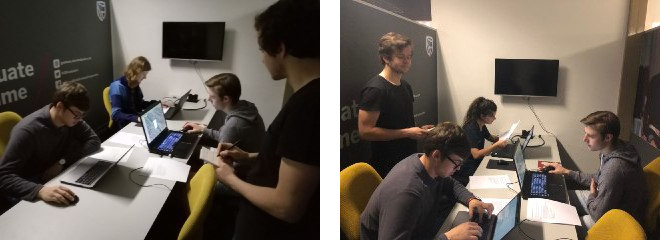
\includegraphics[scale=0.55]{UsabilityTest}
        \caption{Usability test in progress}
        \label{fig:usability}
    \end{figure}

    \newpage
    
    %===========================================================================

    \section{Mobile App Testing}
    \label{sec:mobile-app}

    This section describes the testing policies adopted in the \texttt{web-app}
    repository. The tools used for testing are described in Section
    \ref{sec:ma-tools}.  The layout of the test cases and history of the tests
    are shown respectively in Sections \ref{sec:ma-cases} and \ref{sec:ma-hist}.

    \subsection{Tools}
    \label{sec:ma-tools}

    The mobile app uses JUnit to test various functionality of the app. The built-in test  functionality of Android Studio is used to automate the testing process. The tests can be run by selecting UnitTests in the build options (i.e. the same way as the mobile application would normally be built). This method is used for simplicity and ease of use for example: when change are made to the app, the developer can make the changes and run the tests afterwards to ensure the core functionality is still working. In section \ref{sec:ma-hist}, the tests can be seen

    \subsection{Test Cases}
    \label{sec:ma-cases}

    The tests are in the following location:
    \\
    \\
  	/mobile-app/app/src/test/java/recrec/golfcourseviewer/UnitTest.java

    \subsection{History}
    \label{sec:ma-hist}

    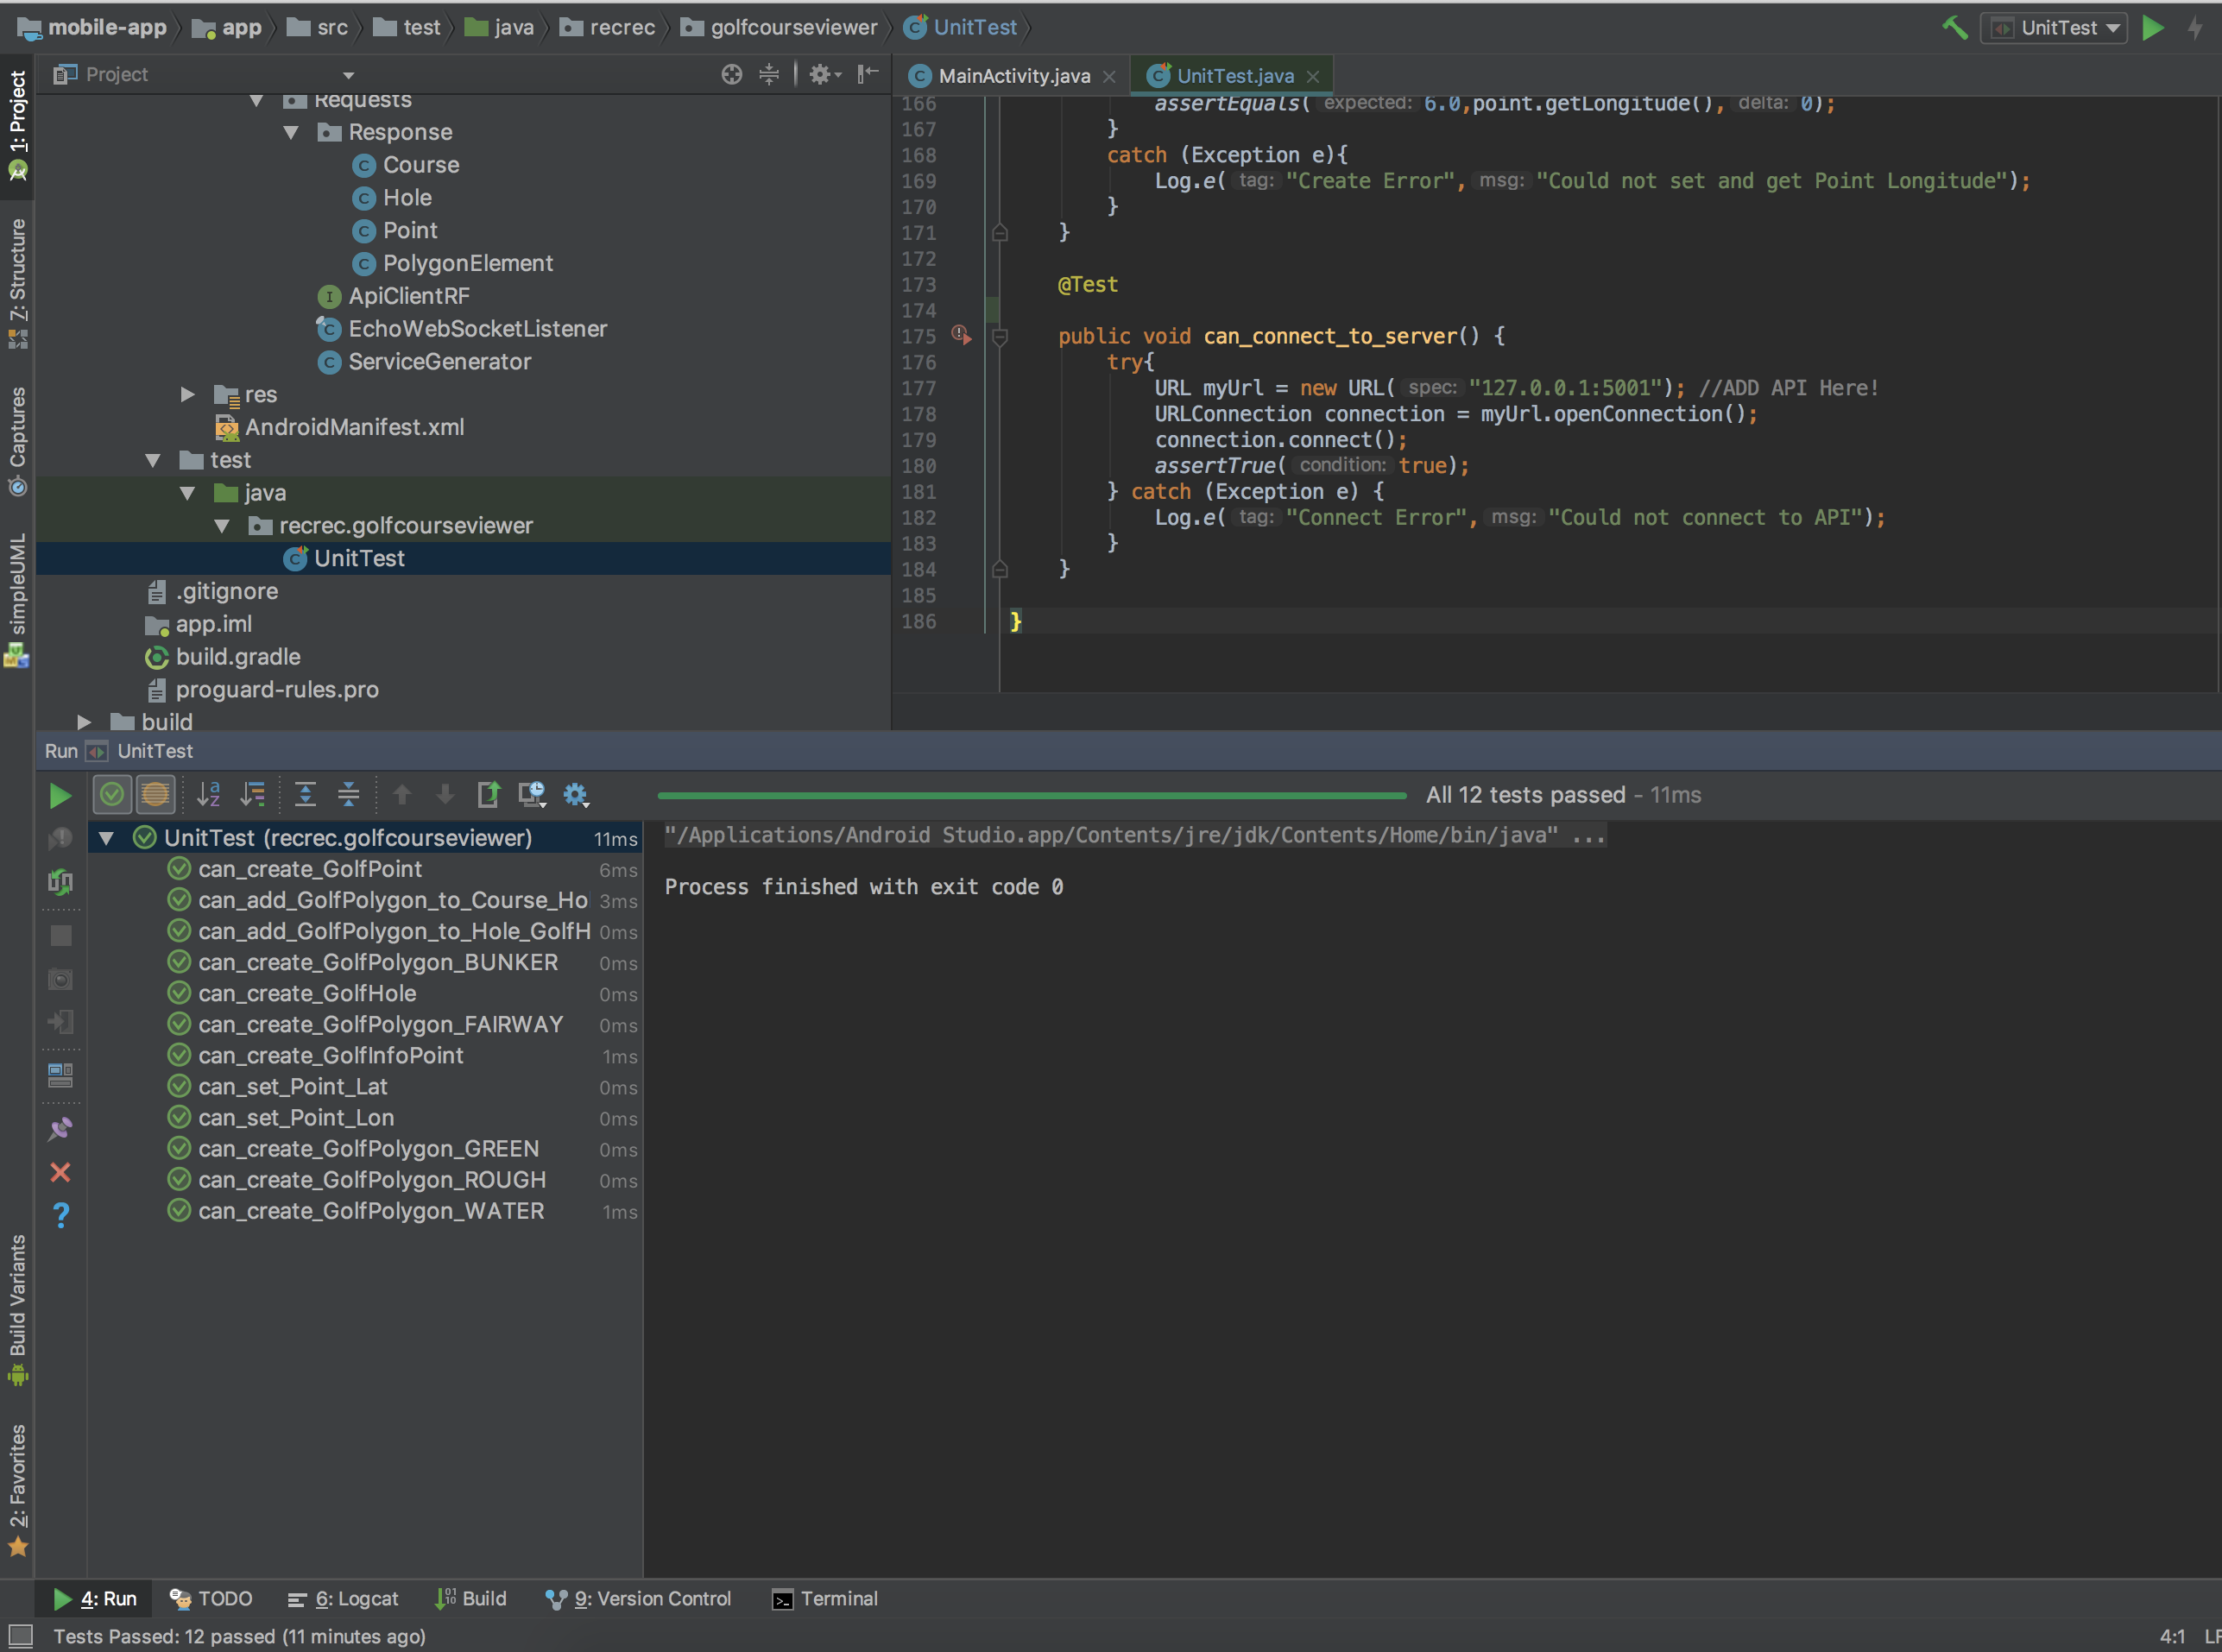
\includegraphics[scale=0.35]{AppTest}

    \newpage

    %===========================================================================

    \section{Mapper API Testing}
    \label{sec:mapper-api}

    This section describes the testing policies adopted in the \texttt{web-app}
    repository. The tools used for testing are described in Section
    \ref{sec:api-tools}.  The layout of the test cases and history of the tests
    are shown respectively in Sections \ref{sec:api-cases} and
    \ref{sec:api-hist}.

    \subsection{Tools}
    \label{sec:api-tools}

    What tool, justify choice and give configuration details (how to use)\ldots

    \subsection{Test Cases}
    \label{sec:api-cases}

    Where (folder) are the tests located\ldots

    \subsection{History}
    \label{sec:api-hist}

    Screenshots\ldots

\end{document}
